\chapter{Experimental observation of k/-k correlations in the depletion of a weakly-interacting Bose gas}

The Bogoliubov interacting Bose-gas has been the subject of a large variety of experimental studies (CITATIONS). However, these experiments have mainly focused on measuring the Bogoliubov spectrum of excitations. More than 60 years after the seminal Lee, Huang and Yang paper \cite{lee1957}, an experimental study of the correlations in the many-body ground-state is yet to be done. As we have seen thus far, our experimental setup is perfectly suited for such an investigation. 

We will detail in this chapter the details of our experiment aiming at detecting \kmk pairs in the depletion of a weakly-interacting Bose gas and our main results. COMPLETER AVEC PLAN?

\section{Numerical procedure to measure two-body correlations}

Our goal is to compute the normalized second-order correlation function:

\begin{equation}
    g^{(2)} (\bm{k},\bm{k'}) = \frac{\mean{\hat{a}^{\dagger}(\bm{k}) \hat{a}^{\dagger}(\bm{k'}) \hat{a}(\bm{k}) \hat{a}(\bm{k'})}}{\mean{\hat{a}^{\dagger}(\bm{k}) \hat{a}(\bm{k}) } \mean{\hat{a}^{\dagger}(\bm{k'}) \hat{a}(\bm{k'}) }}
\end{equation}

We recognize that $\mean{\hat{a}^{\dagger}(\bm{k}) \hat{a}(\bm{k})}$ is the momentum density in mode $\bm{k}$ that we will write $\rho(\bm{k})$ in the following. As seen on the previous chapter, the $\gtwo$ function will take values different from 1 in two cases:

\begin{itemize}
    \item For $\bm{k'} \simeq \bm{k}$, the \textbf{normal} correlations corresponding to the Hanbury Brown and Twiss effect also known as bosonic bunching.
    \item For $\bm{k'} \simeq -\bm{k}$, the \textbf{anomalous} correlations corresponding to the \kmk pairs in the quantum depletion.
\end{itemize}

In practice, plotting the $\gtwo$ function defined as such does not make much sense. On the one hand, the function here is 6D and thus hard to plot in an intelligible way. On the other hand, obtaining a sufficient signal to noise ratio to make correlation measurements for single values of $\bm{k}$ and $\bm{k'}$ is impossible. The idea is then to integrate the $\gtwo$ over all momenta $\bm{k}$ and introduce a new parameter $\delta \bm{k}$ to write:

\begin{equation}
    g_{N,A}^{(2)} (\delta {\bm k})=\frac{\int_{\Omega_{k}} \langle \hat{a}^{\dagger}({\bm k}) \hat{a}^{\dagger}(\delta {\bm k} \pm {\bm k}) \hat{a}({\bm k}) \hat{a}(\delta {\bm k} \pm {\bm k}) \rangle \mathrm{d}{\bm k}}{\int_{\Omega_{k}} \rho({\bm k}) \rho(\delta {\bm k} \pm {\bm k}) \mathrm{d}\bm{k}},
    \label{Eq:g2}
\end{equation}

With this definition, we see that for $\delta \bm{k}=0$, we are either looking at \textbf{normal} \kk correlations (subscript N) when chosing the plus sign, or \textbf{anomalous} \kmk correlations (subscript A) with the minus sign. We reduced the 6D function to a 3D function of $\delta \bm{k}$ which equals $\bm{0}$ when the correlation condition $\bm{k'} = \pm \bm{k}$ is fulfilled. This gives us a natural way to evaluate $\gtwo (\delta \bm{k})$ with the experimental data: we compute the values of the parameter $\delta \bm{k}$ for every detected atom pairs in an experimental run by calculating their momentum difference or sum, for normal and anomalous correlations respectively. By computing the histogram of these values and averaging over many experimental runs, we evaluate the numerator of equation \ref{Eq:g2}.

\subsection{Description of the algorithm}

The algorithm described here is similar to the one used in our previous work \cite{carcy2019momentum,cayla2020} and detailed in \cite{cayla_these,carcy_these}. This previous version was mainly designed for the observation of bosonic bunching. I adapted the algorithm to make it suitable for the calculation of \kmk correlations as well, as we will discuss now.

\subsubsection{Numerator calculation}

The first step is to compute the numerator of equation \ref{Eq:g2} that we denote $G^{(2)}(\delta \bm{k})$. We note $N_{runs}$ the number of experimental runs and $N_{i}$ the number of atoms in the $i$-th shot. The procedure is as follows:

% \begin{algorithm}
% \caption{$G^{(2)}$ calculation}
%     \begin{algorithmic}{}
%         \FOR{$i=1:N_{runs}$}
%             \FOR{$j=1:N_{i}$}
%                 \STATE Compute $\vec{k}_i+\vec{k}_j$
%                 \STATE Increment histogram $G^{(2)}$ corresponding pixel
%             \ENDFOR
%         \ENDFOR
%     \end{algorithmic}{}
% \end{algorithm}

\begin{algorithm}
 \caption{$G^{(2)}$ calculation}
    \begin{algorithmic}
         \For{$i=1:N_{runs}$}
            \For{$j=1:N_{i}$}
               \For{$p=1:N_{i}$}
                    \State Compute $\delta \bm{k} = \bm{k}_j \pm \bm{k}_p$
                    \State Increment 3D histogram $G^{(2)}$ corresponding pixel
                \EndFor
            \EndFor
        \EndFor
\end{algorithmic}

\end{algorithm}

We end up with a 3D histogram where each voxel is associated to a value of $\delta \bm{k} = (\delta k_x,\delta k_y, \delta k_z)$ and records how many atom pairs have this specific momentum sum or difference, depending on the kind of the correlations we want to probe.

The major difference with the previous version of the algorithm is that we record here the full 3D histogram of calculated $\delta \bm{k}$ on every pair of atoms. The procedure was made originally made simpler by calculating three one-dimensional histograms, one for each direction space. For instance, the $x$ direction histogram was obtained by selecting one atom and calculating $\delta k_x$ only for atoms with $k_y$ and $k_z$ close to the one of the considered atom (\textcolor{red}{NUL}). This method obviously saves computing time and RAM space, but is not suited to computing \kmk correlations.

At this point, we record in the central voxels associated to $\delta \bm{k} \simeq \bm{0}$ what we call \textbf{true coincidences}, namely two atoms detected conjointly as a result of \kmk pairing or bosonic bunching. However, we also record \textbf{accidental coincidences} that do not represent correlations but result from the distribution of the atoms. We then need a normalization process to get rid of the contribution of accidental coincidences. 

\subsubsection{Denominator calculation}

We now want to compute the denominator of equation \ref{Eq:g2}, representing the effect of accidental coincidences. To perform this calculation, we would like to have a sample of atoms with the same momentum density than our experimental data but uncorrelated. This can be done by merging all experimental shots, not correlated with one another. We then apply the procedure we have just described to this data set. However, some of the correlations happening in single shots will remain in this large file. In the end, the total number of correlations in the numerator is $\sum_i N_i^2$ whereas the number of coincidences in the merged file is $(\sum_i N_i)^2$. If we note $\bar{N}$ the mean number of atoms per shot, we see that :

\begin{equation}
      \frac{\sum_i N_i^2}{(\sum_i N_i)^2}=\frac{N_{\rm{runs}} \bar{N}^2}{N_{\rm{runs}}^2 \bar{N}^2}=\frac{1}{N_{\rm{runs}}}
\end{equation}{}

Therefore, with enough shots, the contribution of residual coincidences in the denominator is negligible. 

In the end, the integrated $g^{(2)}$ function can obtained by dividing the calculated numerator by the denominator and multiplying by the normalization factor $\frac{(\sum_i N_i)^2}{\sum_i N_i^2}$ taking into account the number of coincidences of the numerator and denominator. Usually, we only take a fraction of all atoms for the denominator calculation to avoid large computation time. 

\subsection{Benchmarking of the algorithm with two-body collision spheres}

Before using the algorithm to look for a supposedly small \kmk pairing signal in the depletion of a weakly-interacting Bose gas, it was crucial to test it on a data set with a large number of \kmk pairs to certify that it was working properly. Luckily, we could re-use the data taken for measuring two-body collisions during the time-of flight described in Chapter 2. The simplest case is to use only one of the lattice beam to induce 1D diffraction and observe only two collision spheres. FINIR


\section{Accessing the BEC depletion}

In order to detect \kmk pairs in the depletion, it is absolutely crucial to remove from the analysis all atoms belonging to the BEC and its diffracted copies showing no correlations as it is a pure coherent state. These atoms indeed largely outnumber the depleted atoms and will therefore entirely drown out the \kmk correlation signal of the quantum depletion, would they not be removed. 
For each recorded data set, we begin the analysis by removing all atoms outside the volume $\Omega_k$ that we design to exclude momentum regions with condensed atoms as illustrated on Fig-\ref{fig:omega_k}. We set $\Omega_k$ to have a cubic symmetry that matches the symmetry of the momentum distribution in a cubic lattice. We remove all atoms with $|k_i| < k_{\rm{min}}$ and $|k_i| > k_{\rm{max}}$ where $k_i$ is the momentum projection along an axis $i=x,y,z$. We use $k_{\rm{min}}=0.15 \, k_d$, corresponding to $\sim 6$ times the RMS width of the BEC peaks, in order to ensure that all condensed atoms have been removed. The high limit is set to $k_{\rm{max}}=0.85 \, k_d$ to exclude higher order peaks and is slightly smaller than the momentum range probed by the MCP.

\begin{figure}
    \centering
    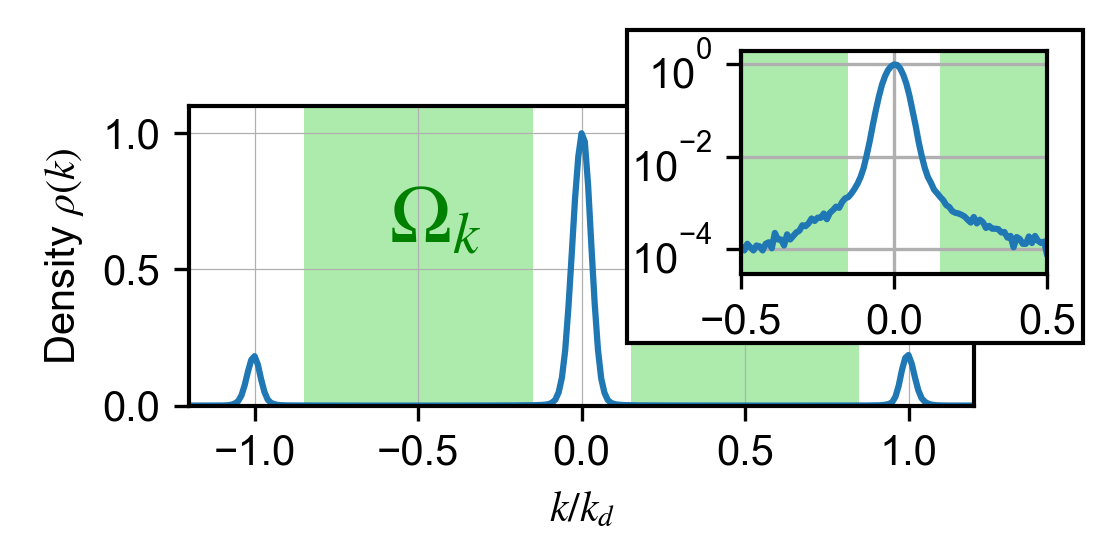
\includegraphics[width=\textwidth]{Fig/Chapter4/densite.png}
    \caption{1D cut of the momentum density illustrating the integration volume $\Omega_k$. The central peak corresponds to the BEC and the lateral peaks at $\pm \ k_d$ to diffraction peaks induced by the presence of the optical lattice. The green area shows the volume $\Omega_k$ containing the depleted atoms selected for the correlation measurement. While barely visible in linear scale, they can be seen in the log scale plot shown in inset.}
    \label{fig:omega_k}
\end{figure}


\section{Observation of the pair correlation signal}

\subsection{Experimental parameters}

We prepare a BEC with a target number of $\NBEC=5 \times 10^3$ atoms in an optical lattice of amplitude $V=7.75 \ E_r$. With this lattice amplitude, we are in the superfluid domain of the phase diagram in which we expect the \kmk correlations. In order to have sufficient statistics, we repeat the experiment $\sim 4,000$ times. In practice, we cannot prepare BECs with the exact same number of atoms at each shot. We then need to post-select the data and remove runs with a detected atom number falling too far from the target number. We allow for $30 \%$ fluctuations around the target number and end up conserving around $\sim 2,000$ runs.

\subsection{$g^{(2)}_A$ correlation function}

We have plotted on Fig-\ref{fig:kmk_signal} 1D cuts through the $g_{A}^{(2)}$ function on which we can see clear correlation peaks standing out from the noise! At this point, we must stress out that the novelty of this signal is that it is the first experimental observation of \kmk pairs in an \textbf{at-equilibrium system}. They have indeed been numerous observations of \kmk pairs, but always in \textbf{out-of-equilibrium} configurations. To a cite a few examples:

\begin{itemize}
    \item Parametric down conversion in quantum optics \cite{burnham1970}.
    \item Dissociation of diatomic molecules in atomic physics \cite{greiner2005}.
    \item Elastic collisions in high energy physics \cite{arnison1982} or with ultracold atoms \cite{perrin2007observation}.
\end{itemize}

\begin{figure}
    \centering
    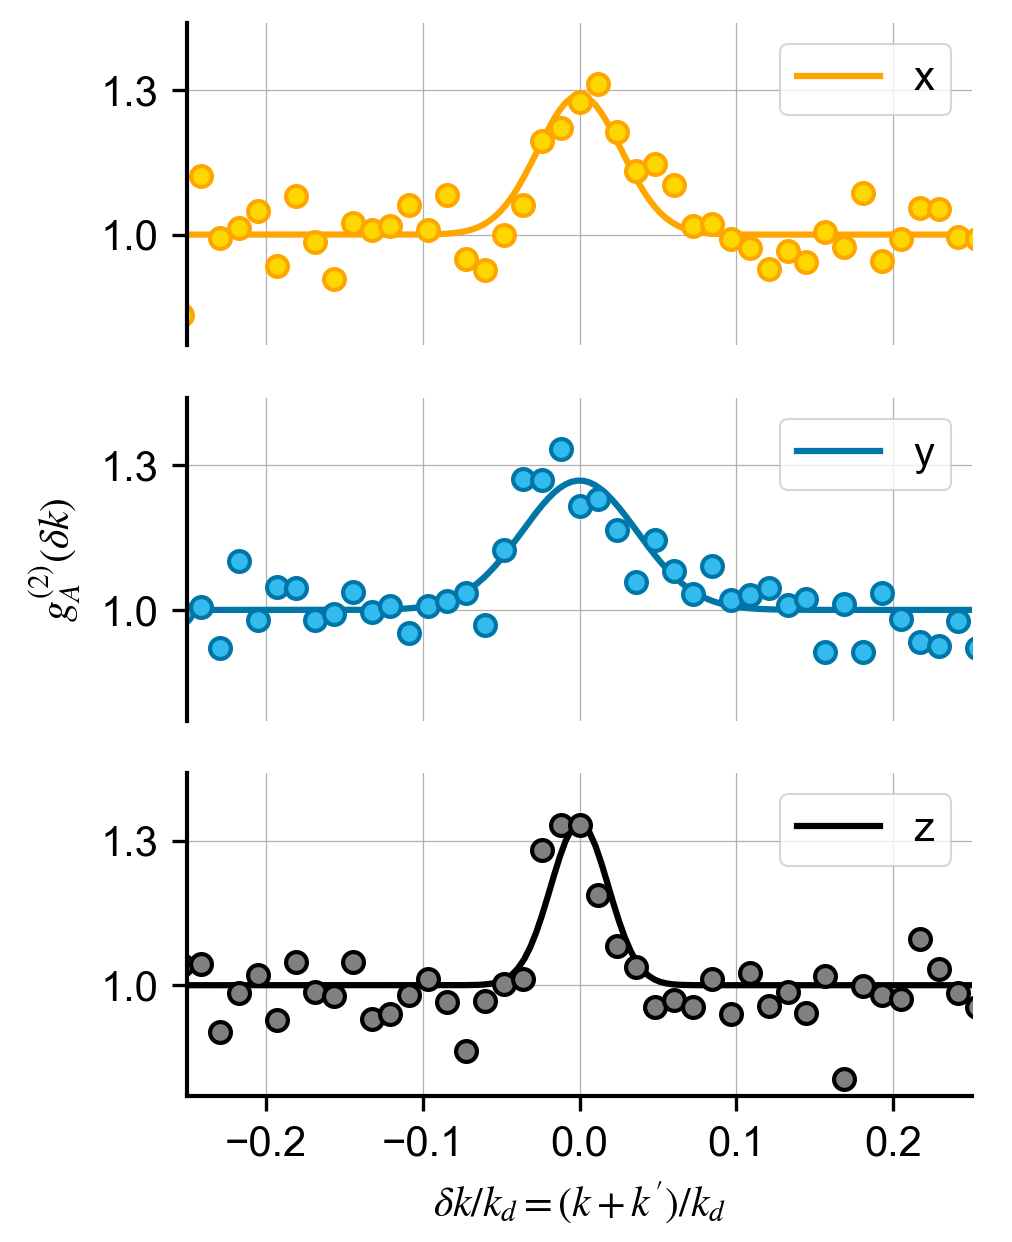
\includegraphics[width=0.65\textwidth]{Fig/Chapter4/1d_cuts.png}
    \caption{1D cuts through $g_{A}^{(2)} (\delta {\bm k})$ along the axis of the 3D optical lattice. The transverse integration is $\Delta k_{\perp}=3 \times 10^{-2} \ k_d$ and the longitudinal pixel size is $\Delta k_{\parallel}=1.2 \times 10^{-2} \ k_d$. The data is fitted by Gaussian functions (solid lines). The nice correlation peaks signal the presence of \kmk pairs.}
    \label{fig:kmk_signal}
\end{figure}

In our experiment, the \kmk pairs are present in an at-rest BEC and are predicted to be populated through the interplay between interactions and quantum fluctuations for which we cannot draw any classical picture.

As we have seen in the previous chapter, the \kmk pairs results from $T=0$ quantum coherences and are expected to be destroyed by temperature. We will now test this prediction experimentally to confirm the origin of the correlation signal.

\section{Effect of temperature}

The temperature can be increased in a rather simple manner by holding the atoms at the final amplitude for a longer duration, the gas being continuously heated over time (attributed to imperfections such as spontaneous emission or mechanical vibrations). We repeat the experiment with a holding time of $500 \ \rm{ms}$ corresponding to hundreds of tunneling times $225 \times h/J$. The increase in temperature can be seen by looking at the momentum density profile as shown in the panel b) of Fig-\ref{fig:kmk_temperature}. As expected, the thermal depletion has increased, increasing the momentum density in the depletion region. Note however that we did not increase the temperature too much to keep a significant condensed fraction of the order of $f_c = 29 \%$ not to entirely remove the quantum depletion.

We plot on Fig-\ref{fig:kmk_temperature} panel a) the $\gtwo_A (\delta \bm{k})$ correlation function for the two different temperatures. 

\begin{figure}
    \centering
    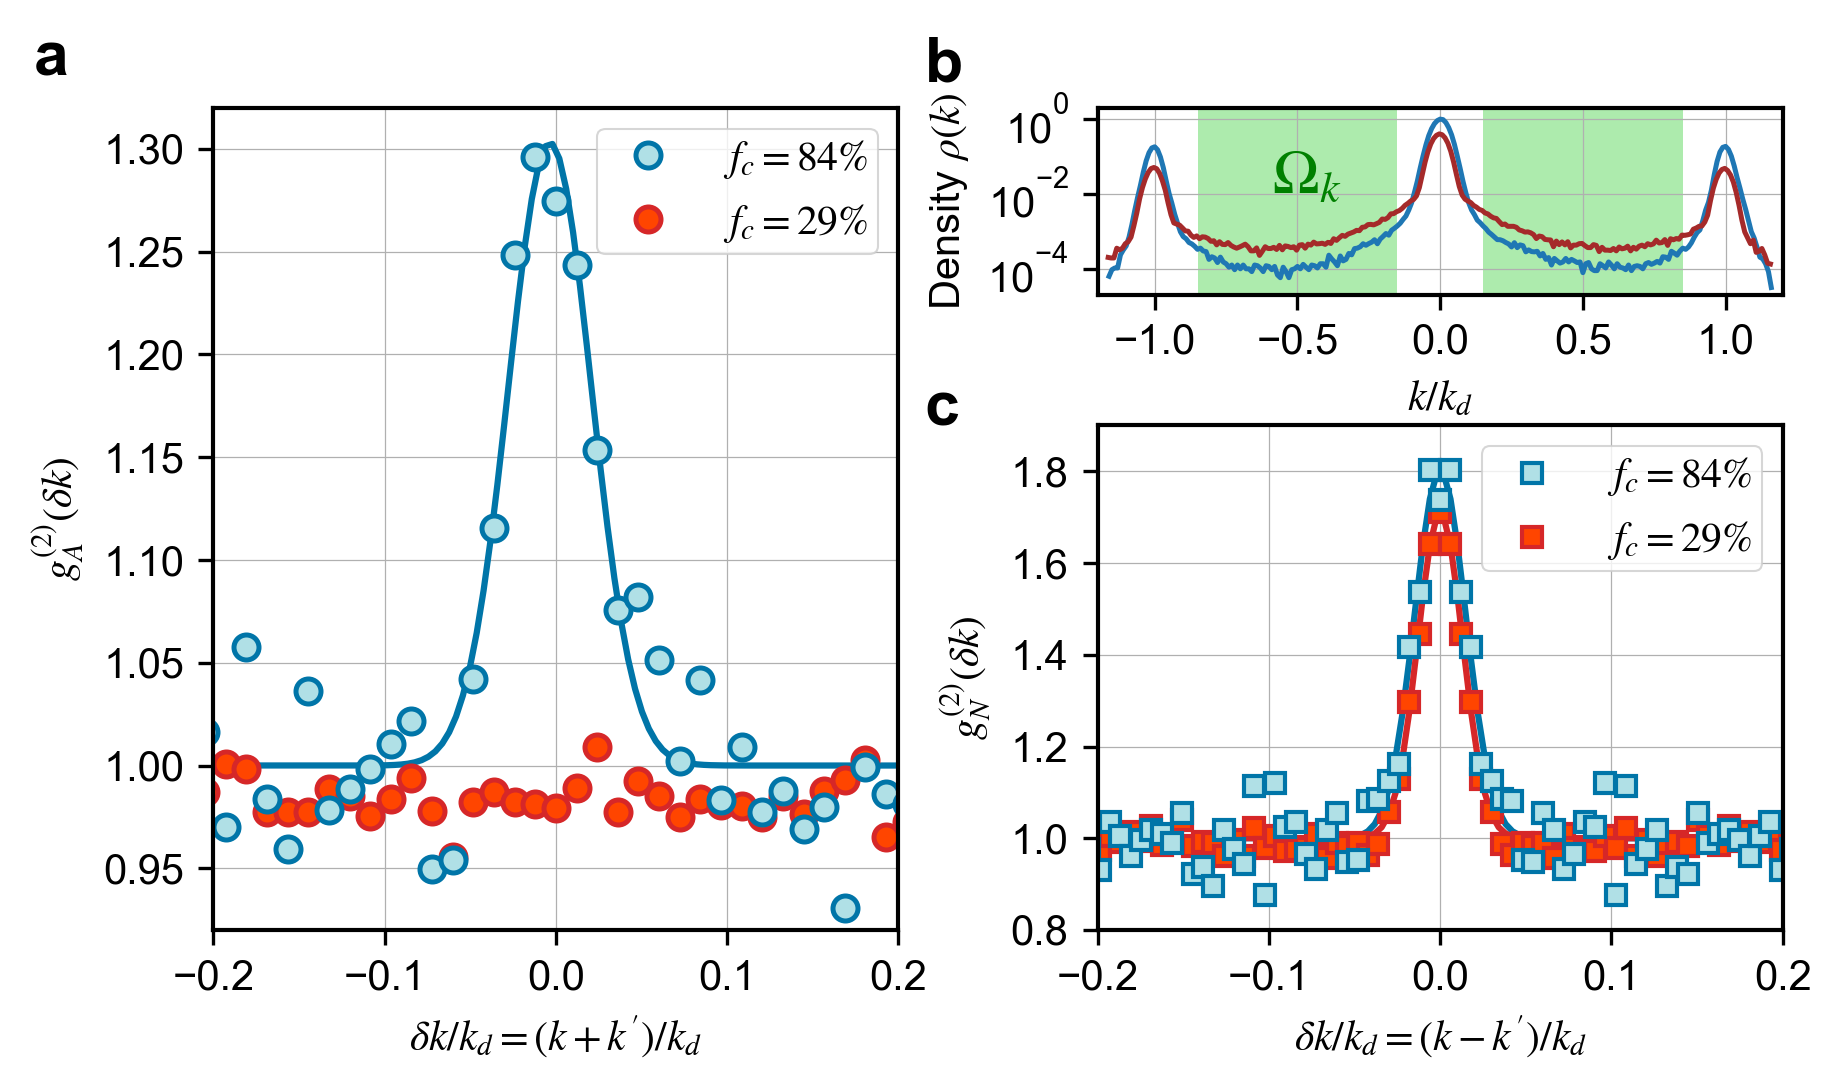
\includegraphics{Fig/Chapter4/kmk_temperature.png}
    \caption{Atom-atom correlations in weakly-interacting BECs at two different temperatures. The data for the low-temperature BEC ($f_{c}=84\%$), {\it resp.} for the heated BEC ($f_{c}=29\%$), are depicted in blue, {\it resp.} in red. 
    {\bf (a)}. Anomalous correlations $g_{A}^{(2)}(\delta k)$ at opposite momenta. The ${\bm k}$/$-{\bm k}$ peak disappears as the temperature increases.
    {\bf (b)}. 1D cut of the density $\rho(k)$ in semilog scale. The depletion density increases with temperature.
    {\bf (c)}. Normal correlations $g_{N}^{(2)}(\delta k)$ for the same datasets and $\Omega_k$. The peak amplitude shows no significant change as the temperature increases. Note that the transverse integration $\Delta k_{\perp}=1.5 \times 10^{-2} \, k_d$ used here reduces the amplitude of the peaks.}
    \label{fig:kmk_temperature}
\end{figure}

\section{Study of the amplitude of the correlation peaks}

\subsection{Transverse integration effects}

\subsection{Scaling with momentum density}

\subsection{Discussion on the detected number of atom pairs}

\section{Study of the width of the correlation peaks}

\section{Relative number squeezing}